\section{Colosso di Pietra}\label{colosso-di-pietra}

Tags: Creatura Creatore: Lorenzo Luogo: Tempio di Naskirophis CR: 5

\section{Colosso di Pietra}\label{colosso-di-pietra-1}

\begin{center}\rule{0.5\linewidth}{0.5pt}\end{center}

\begin{center}\rule{0.5\linewidth}{0.5pt}\end{center}

\textbf{{[}Monster{]}}

\begin{figure}
\centering
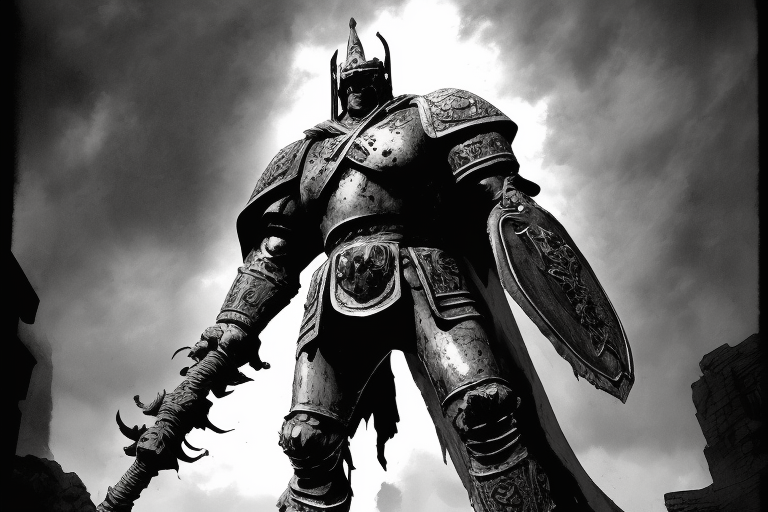
\includegraphics{blkmndy-a-stone-colossus-in-stone-armor-with-stone-sword-and-shield-inside-a-temple-black-and-w_(1).png}
\caption{blkmndy-a-stone-colossus-in-stone-armor-with-stone-sword-and-shield-inside-a-temple-black-and-w
(1).png}
\end{figure}

Informazioni Generali

Dimensione: Grande

Tipo: Costrutto

Attitude:

Velocità di movimento: 30ft

Habitat: Tempio di Naskirophis

Alleati: Naskirophis

Nemesi: Intrusi del Tempio

\begin{center}\rule{0.5\linewidth}{0.5pt}\end{center}

\subsection{1. Descrizione Generale}\label{descrizione-generale}

\begin{center}\rule{0.5\linewidth}{0.5pt}\end{center}

\begin{figure}
\centering
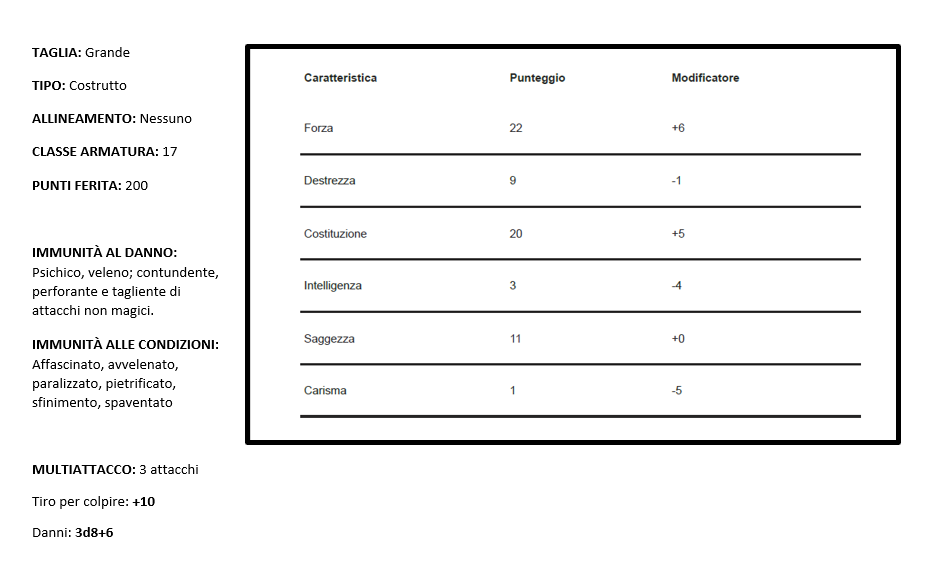
\includegraphics{Screenshot_2023-10-02_145757.png}
\caption{Screenshot 2023-10-02 145757.png}
\end{figure}

Un antico colosso, dalle sembianze di un guerriero in armatura, pronto a
sbarrare la strada a tutti gli intrusi che osano introdursi nel tempio
del suo padrone.

Alto più di 30 metri, ha spalle larghe, un possente petto e arti
muscolosi scolpiti nella roccia stessa. Un elmo corona il suo capo,
mentre una lunga spada e uno scudo massiccio sono stretti tra le sue
mani, pronti per la difesa del tempio.

\subsection{2. Distribuzione e Habitat}\label{distribuzione-e-habitat}

\begin{center}\rule{0.5\linewidth}{0.5pt}\end{center}

Questo colosso è un golem di pietra che si trova nel Tempio di
Naskirophis. Costituisce la seconda sfida da affrontare per chiunque osi
intrufolarsi illegalmente all'interno del sacro luogo.

\subsection{3. Comportamento}\label{comportamento}

\begin{center}\rule{0.5\linewidth}{0.5pt}\end{center}

Il colosso di pietra segue ogni movimento dei suoi nemici con uno
sguardo intenso, pronto a scattare in azione al minimo segno di
intrusione. Tuttavia, il suo comportamento è interamente controllato da
un demone rosso. Questo demone oscuro manovra la marionetta di pietra
con maestria, dirigendo le sue azioni e reagendo agli attacchi degli
intrusi con astuzia spietata.

\subsection{4. Variazioni}\label{variazioni}

\begin{center}\rule{0.5\linewidth}{0.5pt}\end{center}

Il colosso di pietra nel Tempio di Naskirophis è una presenza singolare
e unica, creata per proteggere il tempio dalle intrusioni.

\subsection{5. Interazioni con gli
Umani}\label{interazioni-con-gli-umani}

\begin{center}\rule{0.5\linewidth}{0.5pt}\end{center}

Il compito principale del colosso di pietra è quello di impedire
l'accesso illegale al Tempio di Naskirophis. Ogni creatura che tenta di
attraversare il secondo livello del tempio senza dare la corretta parola
d'ordine è considerata un nemico e viene attaccata senza pietà dal
colosso.
